\newpage\cleardoublepage\phantomsection
\section{Time computation}
\subsection{What do we measure?}
The last processor is always the last to finish since it waits for its predecessors to complete.
The computation time is thus the time span of the last processor.

A more precise computation for the \emph{per process time} computation : passive communication time has not been taken into account.

\subsection{Efficiency}

We can see in \ref{fig:time:1} that the first processor is the one who works most, this is because it includes active communication time, when the first processor is the source of the index broadcast. 

\begin{figure}
	\centering
	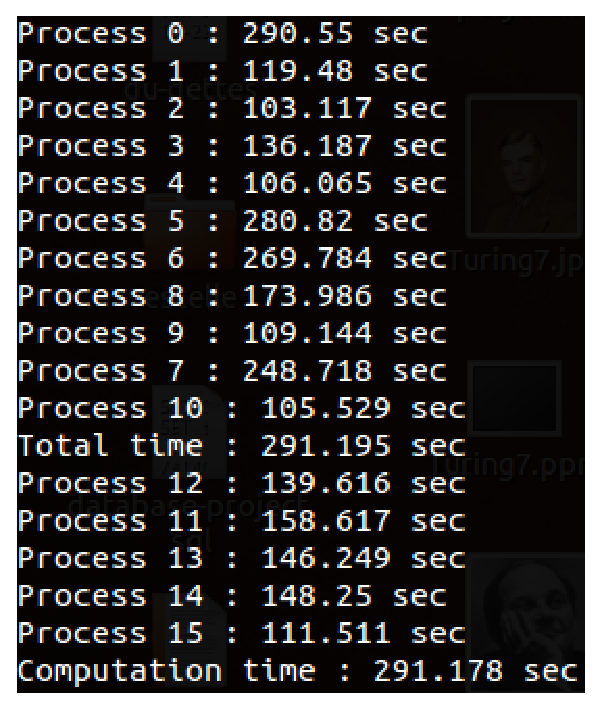
\includegraphics[width=0.4\textwidth]{eps/time}
	\caption{\label{fig:time:1} Computation of the first 10,000,000,000 prime numbers with 16 processors}
\end{figure}

This also shows us that the communication time roughly doubles the time of time spent on the prime generation problem. This could have been improved by grouping the broadcast into a single call (grouping the variables in a byte array), but is still nothing compared to the file writing problem.

\subsection{Conclusion}
Maybe the real bottleneck has arised at the very end of the project. We focused so much time on the prime generation number that the main problem shifted to a file writing problem. The only reasonable approach to tackle this problem is to get rid of the communication between proccessors.